\documentclass[10pt,letterpaper]{article}

% Make everything look pretty
\usepackage{microtype}
\usepackage{graphicx}
\usepackage{color}

% Figs
\usepackage{wrapfig}
\usepackage{epstopdf}
\DeclareGraphicsExtensions{.pdf,.png,.jpg}

% Links
\usepackage{url}
\usepackage[hidelinks]{hyperref}
\usepackage{cite}

% Header/footer/title
%\usepackage{fancyhdr}
%\usepackage{titling}
%\usepackage{lastpage}

\usepackage{titlecaps}

% Set margins
\usepackage[margin=1in]{geometry}
\addtolength{\topmargin}{0.5in}
\addtolength{\textheight}{-0.5in}

% Numbering/labeling of sections and subsections
%\renewcommand\thesubsection{\thesection.\alph{subsection}}
%\renewcommand\thesubsubsection{\thesection.\alph{subsection}.\roman{subsubsection}}

\usepackage{fixltx2e}
\usepackage{float}
\usepackage{url}


\begin{document}

%\title{\titlecap{\scshape Dissertation Proposal} \normalfont \\ \vspace{2 mm}
%Auraglyph: Handwritten Computer Music Programming, Composition and Design}

\title{\titlecap{\scshape Handwritten Computer Music Programming, Composition, and Design} \\ \vspace{2 mm}
\normalfont\large A Dissertation Proposal for the Center for Computer-based Music Theory and Acoustics, Stanford University}

\author{Spencer Salazar}

\maketitle

\begin{figure*}[h!]
	\centering
	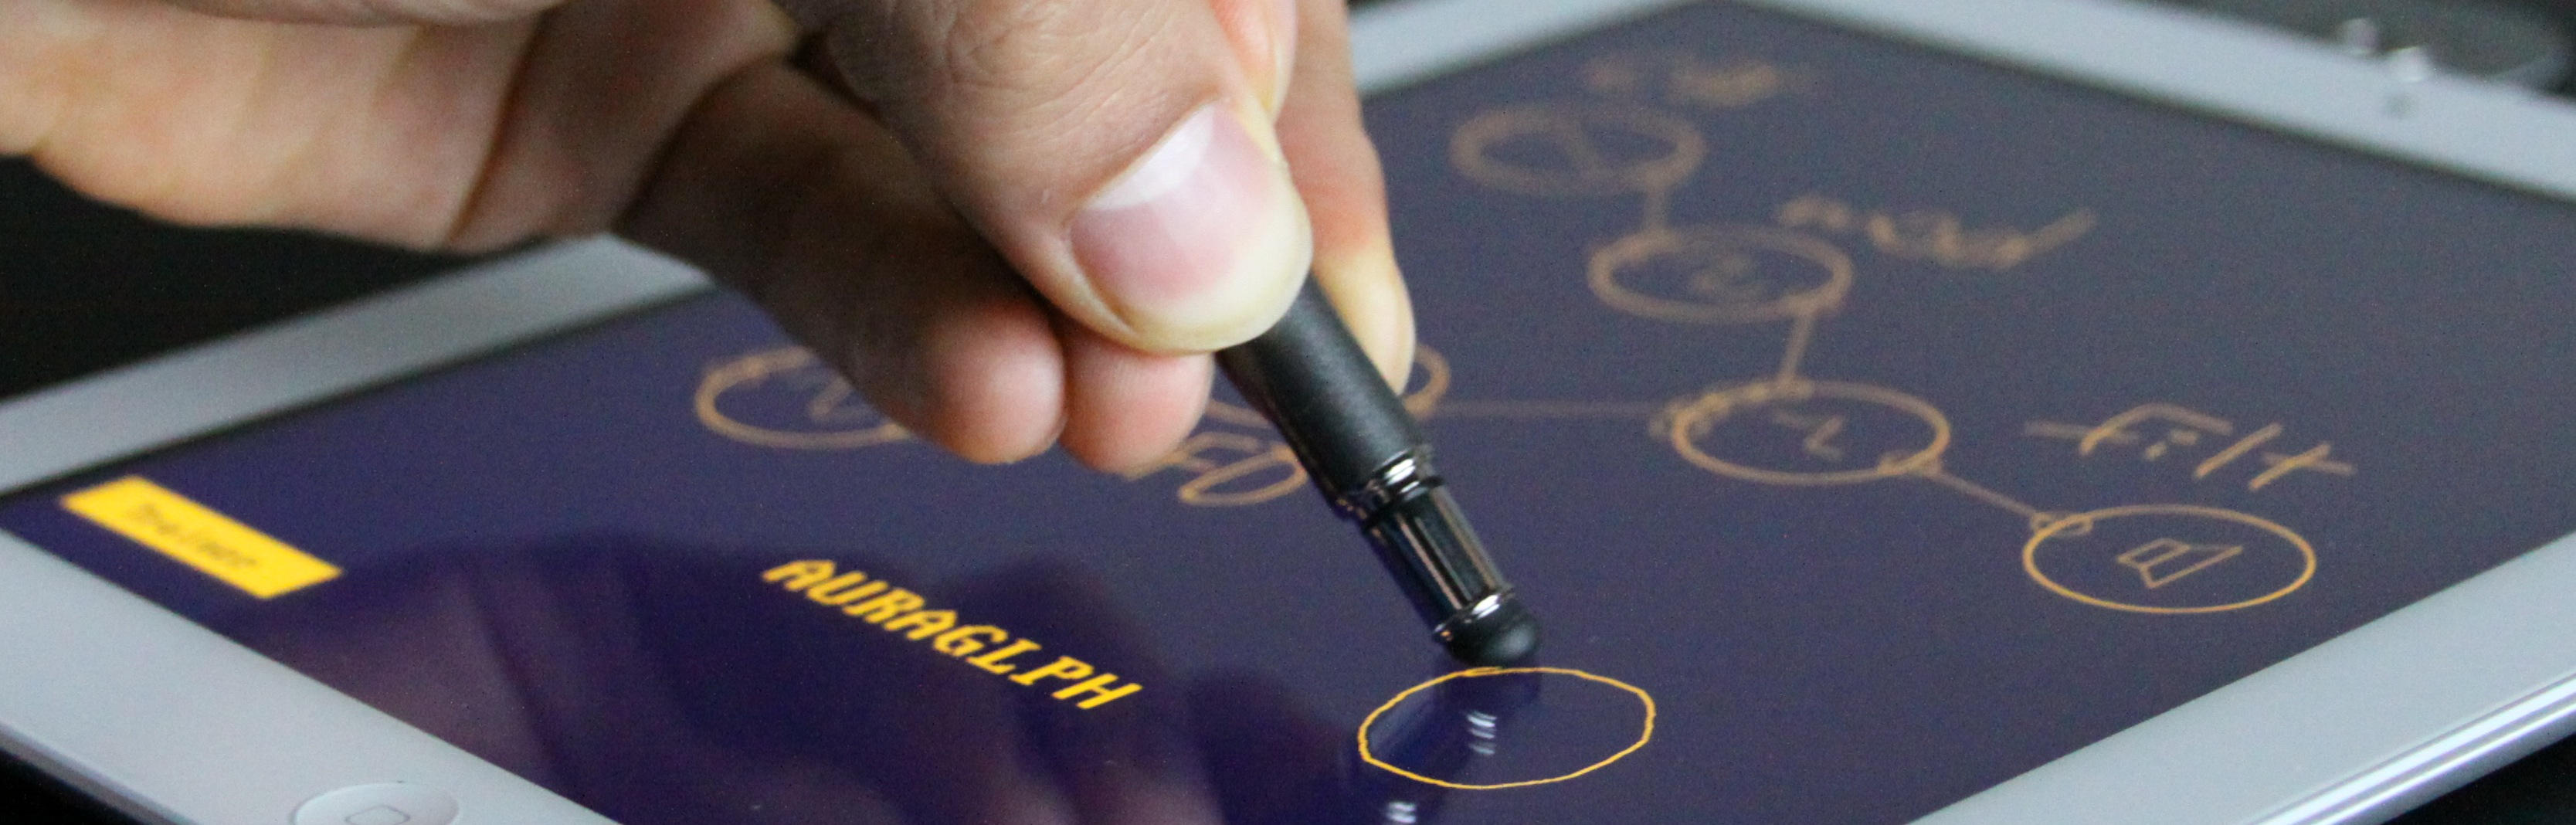
\includegraphics[width=0.9\textwidth]{figures/auraglyphHand2.jpg}
	\caption{Auraglyph, an iPad application developed to demonstrate concepts of handwritten computer music.}
	\label{fig:auraglyphInUse}
\end{figure*}

\section{Introduction}
\label{sec:Introduction}

Touch-based computing has profoundly altered the landscape of mainstream computing in the early 21st century. 
Since the introduction of the iPhone in 2007 and the iPad in 2010, scores of touchscreen devices have entered the popular consciousness -- mobile phones, tablet computers, watches, and desktop computer screens, to name a few. 
New human-computer interaction paradigms have accompanied these hardware developments, addressing the complex shift from classical keyboard-and-mouse computing to multitouch interaction. 

For my dissertation, I propose exploring a new model for touchscreen interaction with musical systems that combines use of stylus-based handwriting input with direct touch manipulation. 
This system might provide a number of advantages over existing touchscreen paradigms for music. 
Stylus input, complemented by modern digital handwriting recognition techniques, replaces the traditional role of keyboard-based text/numeric entry with handwritten letters and numerals.
In this way, handwritten gestures can both set alphanumeric parameters and write out higher level constructs, such as programming code or musical notation. 
A stylus also allows for modal entry of generic shapes and glyphs, e.g. canonical oscillator patterns (sine wave, sawtooth wave, square wave, etc.) or other abstract symbols.
Finally, the stylus provides precise graphical free-form input for data such as filter transfer functions, envelopes, and parameter automation curves. 
In this system, multitouch finger input continues to provide functionality that has become expected of touch-based software, such as direct movement of on-screen objects, interaction with conventional controls (sliders, buttons, etc.), and other manipulations. 
Herein I discuss a proposal for designing, prototyping, and evaluating a system developed according to these concepts, which I have code-named ``Auraglyph.'' 

\begin{figure*}[h!]
	\centering
		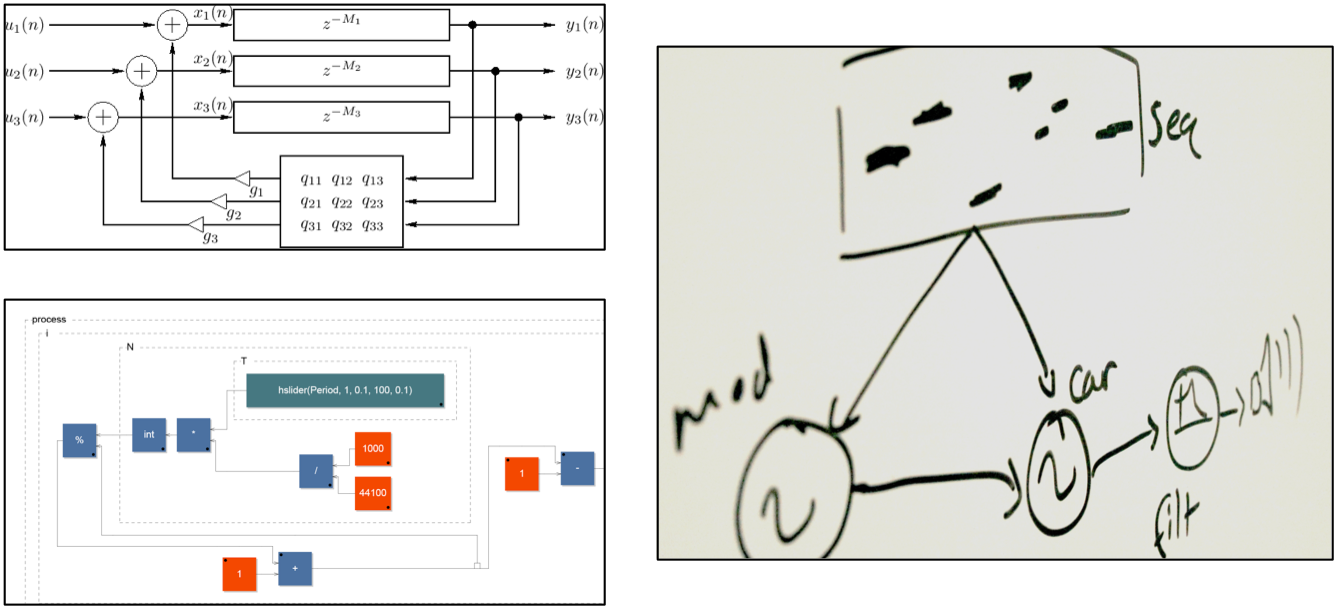
\includegraphics[width=0.9\textwidth]{figures/block.png}
	\caption{Example block diagrams. Top-left: a feedback delay network\protect~\cite{smith2010pasp}. Bottom-left: compiler-generated block diagram from the Faust programming language\protect~\cite{faustOnline}. Right: hand-drawn block diagram.}
	\label{fig:blockDiagram}
\end{figure*}

\section{Related Work}
\label{sec:RelatedWork}

%Touchscreens and music: 
%Handwriting recognition and music: "Exemplar-based learning in adaptive optical music recognition system" (Fujinaga 1996)

In my research, handwriting recognition has previously found little use in interactive computer music. 
Fujinaga et al. explored character recognition of traditional staved musical notation~\cite{fujinaga1989computer, fujinaga1996exemplar}, as have Miyao and Marayuma~\cite{miyao2007online}. 
Direct, graphical manipulation of computational data via pen or stylus, augmented by computer intelligence, goes back as far as Sutherland's Sketchpad~\cite{sutherland1964sketch} and GRAIL and the RAND Tablet by Ellis et al.~\cite{davis1964rand}. 

Object graph-based programming languages such as PureData~\cite{puckette1996pure} and Max/MSP~\cite{zicarelli1998extensible} have tremendously influenced the space of visual computer music design and composition. 
These systems provide both a status quo of graphical music programming and illuminate potential hazards to this approach. 
More recently, the Kronos programming language extended functional programming models to a visual space in the context of real-time music performance~\cite{norilo2012visualization}. 
Mira, an iPad application, dynamically replicates the interface of desktop-based Max/MSP programs, joining conventional music software development with touch interaction~\cite{tarakajian2013anmira}. 
Faust is a text-based functional programming language for designing block diagrams that are compiled to audio processing programs or plugins~\cite{orlarey2009faust}. 

Mobile application developer Smule~\cite{wang2009smule} has built software instruments and music experiences tailored to the characteristic features of mobile devices. 
For instance, Ocarina utilizes the touchscreen, microphone, and accelerometer of a mobile phone to create a unique, compact musical instrument with a network and location-based social aspect~\cite{wang2014ocarina}. 
Leaf Trombone further extends this social aspect with real-time, globablly networked musical interactions for critiquing musical performances~\cite{wang2011world}. 
Magic Fiddle brings these ideas to the iPad, whose larger size accommodates a different set of interactions, such as finer grained pitch control and touch-based amplitude control~\cite{wang2011designing}. 

This proposal has been directly motivated by developments in the ChucK programming language~\cite{wang2008chuck}. 
Efforts to work with ChucK code on mobile touchscreen interfaces has led to porting miniAudicle, ChucK's dedicated development environment~\cite{salazar2006miniaudicle}, to the iPad. 
However, writing ChucK code with a touchscreen virtual keyboard has proven so far to be unnatural and generally inferior to conventional keyboard-based coding. 
Similarly, the popular desktop music programming environments SuperCollider~\cite{mccartney2002supercollider} and PureData exist in mobile software primarily as backend audio engines rather than full-fledged software development interfaces.   

\section{Handwritten Computer Music}
\label{sec:HandwrittenComputerMusic}

This proposal is motivated by the desire to better understand the distinguishing capabilities and limitations of touchscreen technology, and, using these as guiding principles, to enable expressive music interactions on such devices. 
Complex software developed for a given interaction model --- such as keyboard-and-mouse --- may not successfully cross over to a different interaction model --- such as a touchscreen device. 

The initial insight leading to this proposal was that numeric and text input on a touchscreen might be more effectively handled by recognizing hand-drawn numerals and letters, rather than an on-screen keyboard. 
I soon realized that handwriting recognition could also handle a substantial number of handwritten figures and objects beyond just letters and numbers. 
A user might then draw entire object graphs and audio topologies to be realized as an audio system or musical composition, in real-time, by the underlying software application. 
Such a system might even be extended to support actual software programming via handwriting. 

From here a natural metaphor for interaction arose, that of a handwritten block diagram.
In both computer-generated and manually produced variants, block diagrams are utilized extensively in digital audio and computer music development processes (Figure \ref{fig:blockDiagram}). 
We would like users of our system to feel as if they are drawing a block diagram of their musical system on a whiteboard or sheet of paper, and then for the software to manifest that design. 

This metaphor provides several notable benefits. 
Writing and drawing with a pen or pencil on a flat surface is a foundational interaction for an incredible number of individuals, as this activity is continuously developed from early education around the world. 
Moreover,  perhaps the ultimate goal of software interfaces is to simplify the mapping between the user's conceptual abstraction of an idea and the translation of that idea to a digital representation. 
The extent to which this goal is met determines the ease of a user successfully inputting their parameters to the software and interpreting its output. 
The block diagram is a pervasive conceptual abstraction, produced for education (Figure \ref{fig:blockDiagram}, top-left, was taken from a text book), system design (Figure \ref{fig:blockDiagram}, right), and numerous other applications, despite that creating these diagrams is rarely necessary for actually building the represented system. 
Therefore, a block diagram-oriented design system, with a pen-and-paper interaction metaphor, goes great lengths towards diminishing the distance between human thought process and digital construct. 

\section{Auraglyph}
\label{sec:Auraglyph}

The primary tangible goal of this dissertation is to produce a complete software environment demonstrating the core principles of handwritten computer music. 
The working prototype of this environment is called \emph{Auraglyph}. 

A high-level model of interacting with Auraglyph is shown in Figure \ref{fig:auraglyphSystem}. 
The user's viewpoint is represented by the iPad in the center, acting as a window into a larger system. 
This viewpoint may be freely moved about the space using conventional gestures (swipe, pinch) to scroll and zoom throughout the space. 
The lower plane, extending infinitely in two dimensions, contains control logic, programming code, and unit generators, comprising the bulk of an Auraglyph program's functionality.
Some unit generators may contain an internal network of logic and ugens designed by the user, and the contents of these may be examined by further zooming in to the container ugen.  
The upper plane contains user interface controls, which have been defined in the main programming area. 
This plane exists primarily for interacting with these controls, allowing Auraglyph programs to present a clearly defined interface. 


\begin{figure*}[h!]
	\centering
		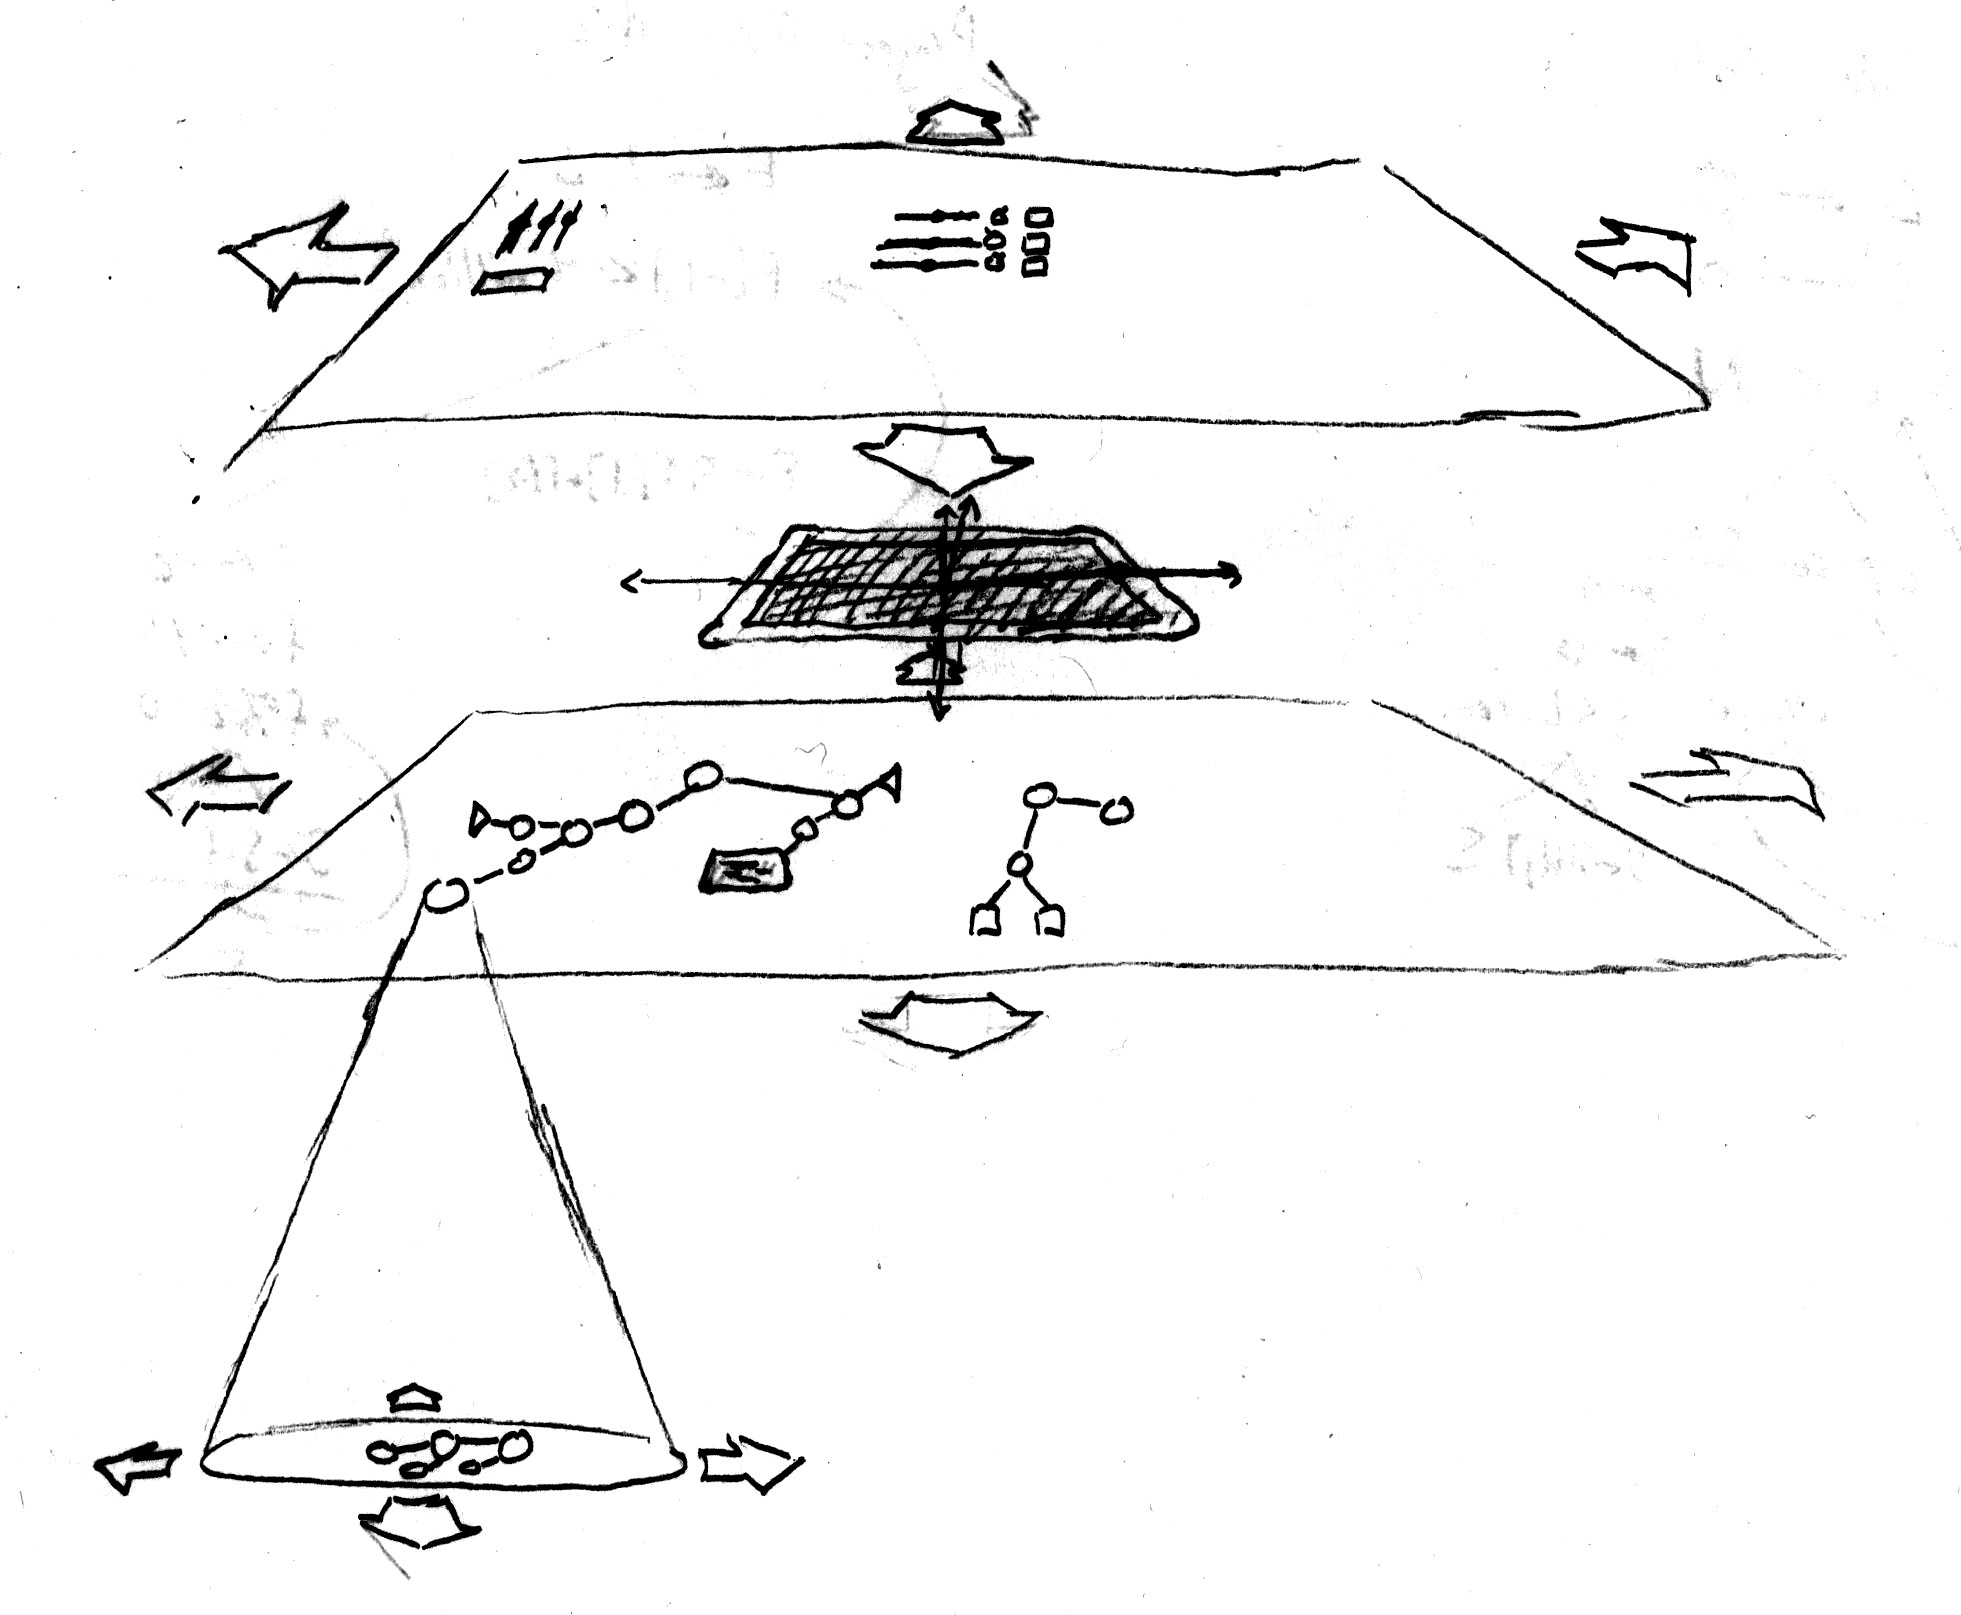
\includegraphics[width=0.9\textwidth]{figures/HWCM-model.jpeg}
	\caption{High-level model of Auraglyph interaction. }
	\label{fig:auraglyphSystem}
\end{figure*}

The functional elements of an Auraglyph program are divided into visual audio units and textual programming code. 
Audio units include conventional unit generators and other related control units, such as timers, control curves, data converters, and sequencers. 
These are created as they are drawn by the user, via stylus input. 
First, the user draws the basic outline of a unit --- a circle --- on the lower plane's canvas, indicating that he or she would like a unit at that location. 
Then, the user draws the desired unit type within the circle (e.g. drawing a sine wave constructs a sine oscillator). 
Not all unit types have suitable hand-drawn mnemonics, in which case a menu is also available to select the unit's type. 
Once created, units can be interconnected by drawing connections between them. 
By creating and interconnecting a variety of unit types in this way, complex musical audio networks can be realized. 

Programming code can also be written directly to the canvas (Figure \ref{fig:auraglyphCode}). 
The syntax of the code is specific to Auraglyph, optimized for the unique capabilities and limitations of handwritten stylus input. 
The links between code and audio units may be flexible, but they are well-defined. 
For example, in Figure \ref{fig:auraglyphCode}, the box around the \textit{f1} character indicates that it is part of both programming code and the audio network. 
As this work progresses, the specific requirements and features of the programming language itself will become more clear. 
Presently, languages such as ChucK provide inspiration for the audio-based components of the programming language, and Python, Ruby, and other dynamic languages for general purpose programming. 

\begin{figure*}[h!]
	\centering
		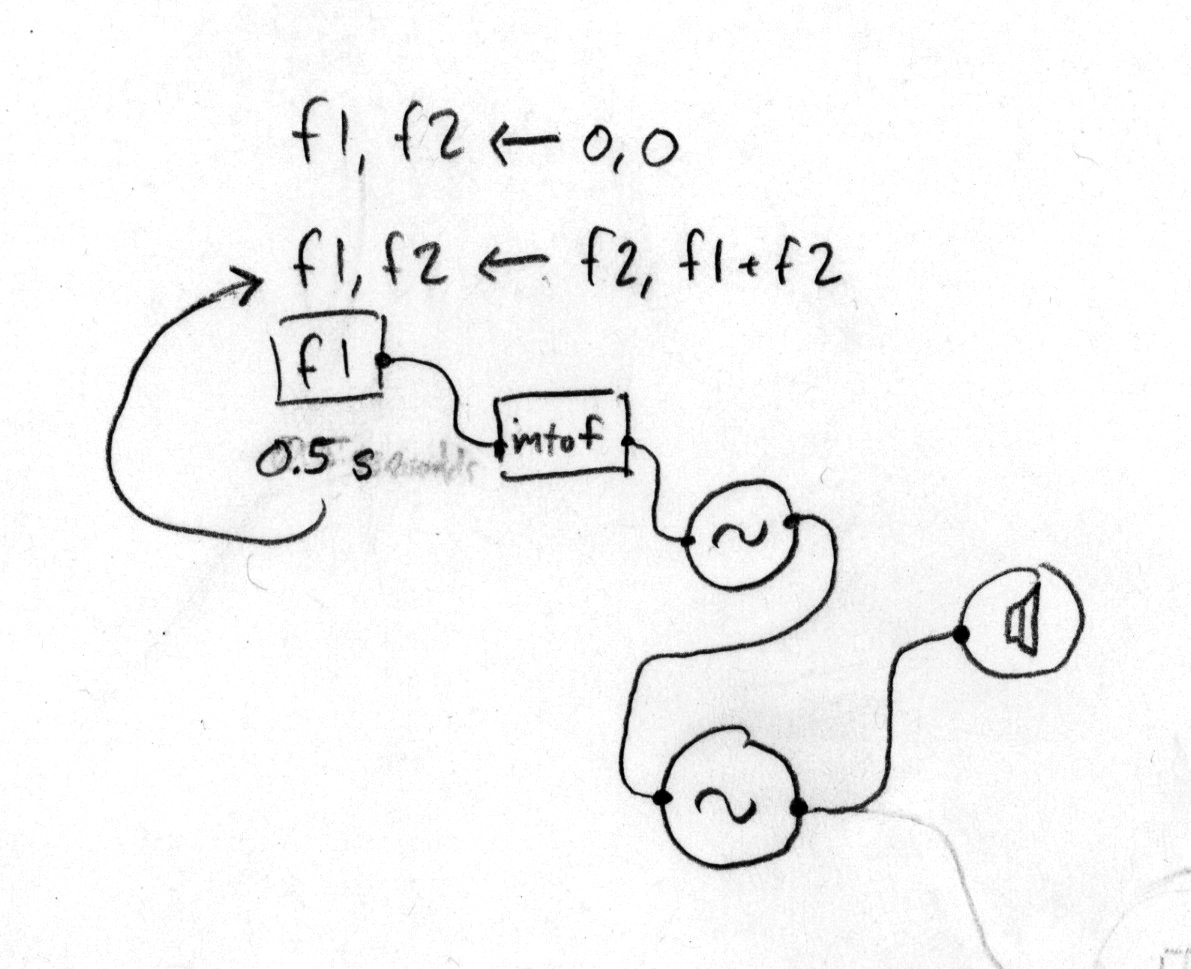
\includegraphics[width=0.9\textwidth]{figures/HWCM-codeblock.jpeg}
	\caption{Example of handwritten code integrated into a unit generator graph. This program chooses notes according to the Fibonacci sequence, selecting a new note every half second. }
	\label{fig:auraglyphCode}
\end{figure*}

In addition to the core system described above, I am interested in additional interactions that are not fundamental to the primary handwritten computer music experience. 

\paragraph{The system facilitates multi-user interactions with objects used to communicate data over the network.} 
Objects might exist to transmit and receive arbitrary control data over OpenSoundControl~\cite{wright1997osc}. 
Additionally they could provide discovery mechanisms for finding other local-area or wide-area Auraglyph users to make music with. 

\paragraph{Stylus input can also be used to hand-write musical notation on staves.}
Snippets of notation data can then be passed around and modified both with traditional list transformations (add/remove, combine, reverse, etc.) and music-specific transformations (transposition, inversion, tuning, etc.). 

\paragraph{Novel stylus designs can provide additional expressivity in this system.}
For example, a stylus with touchscreen-compatible tips on both ends might designate a draw end and an erase end, mimicking the conventional pencil-and-eraser. 
Similarly, multiple styluses might be distinguished and treated differently by this system, allowing for different ``colors.''
Each stylus in this scenario would support a separate interaction. 
Distinguishing stylus input from manual touch input also presents interesting design opportunities. 
Consumer touchscreen styluses generally do not support these features, so specialized styluses may need to be individually constructed to enable these interactions. 

\section{Evaluation}
Of particular interest in exploring these scenarios is Auraglyph's viability as a primary development interface for music software. 
In what scenarios would I rather use Auraglyph than a desktop software application? 
What kind of music can I make with Auraglyph? 
Is the music made with Auraglyph ``good?'' 
Does Auraglyph affect how I think about music and computing, and, if so, how? 
To a significant extent, the answers to these questions form the criteria for success of handwritten computer music. 

Direct user testing may also shed light on the utility of Auraglyph for expressive music software programming. 
Common in the software development industry, this type of design validation gives test users a script of actions to undertake within the program. 
As each user performs these tasks, relevant metrics are gathered, such as time needed to complete each task, the number of errors made before completing a task, and the user's self-reported assessment of the tasks' difficulty. 
These tests could be performed with the same script across both Auraglyph and comparable environments like Max/MSP or ChucK. 
This variety of testing is not conclusive as to any given application's utility or expressiveness, but does allow a quantitative approach that might reasonably suggest its overall quality. 

A related issue is the audience of the software. 
Auraglyph is not necessarily intended for beginners or amateurs (though it would not intentionally discourage them from using it either). 
A primary goal of Auraglyph is to offer the depth of functionality that one might find in popular music software environments. 

%\section{Technical Challenges}
%\label{Technical}

\section{First Draft}
\label{sec:SystemDescription}

I have already developed an initial draft of Auraglyph, thus far embodying a number of the principles stated above. 
A description of this system and the concept of handwritten computer music was submitted to the International Conference on New Interfaces for Musical Expression (NIME) 2014. 

%As a framework to prototype and evaluate the concepts discussed above, and for use in composition and sound design, we developed Auraglyph, a software application for iPad. 
%A user interacts with Auraglyph using an iPad-compatible stylus (many models of which are widely available) and traditional touch interaction. 

\begin{figure}[h]
	\centering
		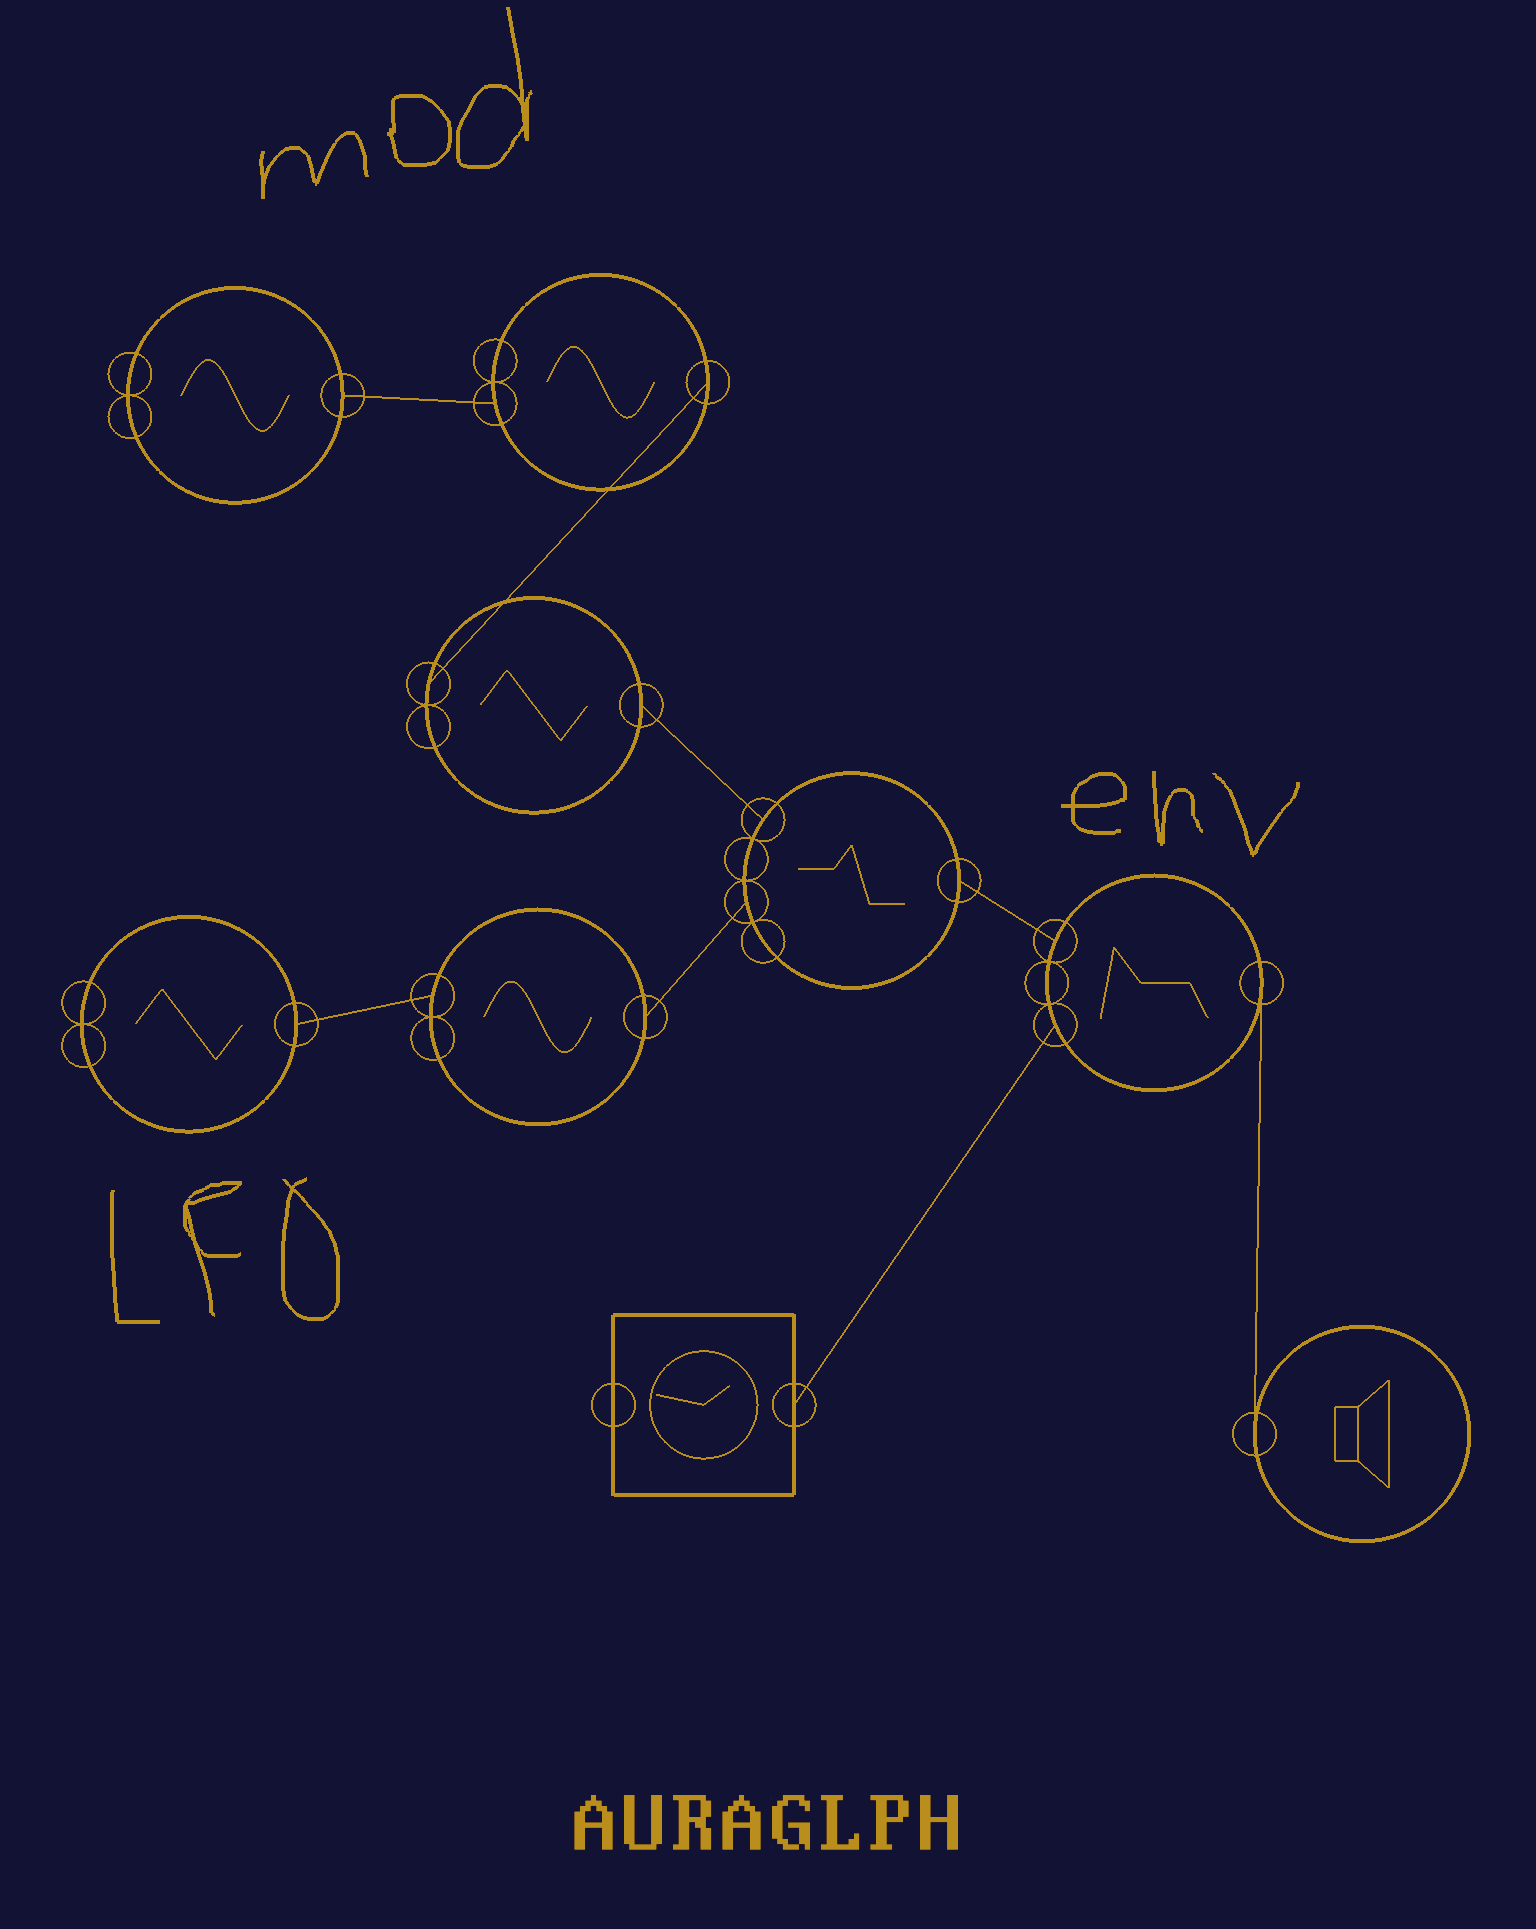
\includegraphics[width=0.45\textwidth]{figures/patch.png}
	\caption{A full Auraglyph patch, with annotations.}
	\label{fig:patch}
\end{figure}

The basic environment of this version of Auraglyph is an open, scrollable canvas in which the user freely draws with a stylus. 
Using a variety of pen strokes, a user creates interactive \emph{objects} (such as unit generators, control rate processors, and input/output controls), sets parameters of these objects, and forms connections between them. 
Collectively, these objects and their interconnections form a \emph{patch}. 
After a user completes a pen stroke (a single contour between touching the pen to the screen and lifting it off the screen), it is matched against the set of base object glyphs available in the main canvas, via a handwriting recognition algorithm. 
Main canvas objects whose glyphs can be matched include an audio rate processor (unit generator), control rate processor, input, or output. 
If the stroke matches an available glyph, the user's stroke is replaced by the actual object. 
Unmatched strokes remain on the canvas, allowing the user to embellish the canvas with freehand drawings. 

Tapping and holding an object will open up a list of parameters for that object (Figure \ref{fig:editor}). 
Selecting a parameter from this list opens a control into which writing a number will set the value. 
This value can then be accepted or discarded, or the user can cancel setting the parameter entirely. 

\begin{figure}[h]
	\centering
		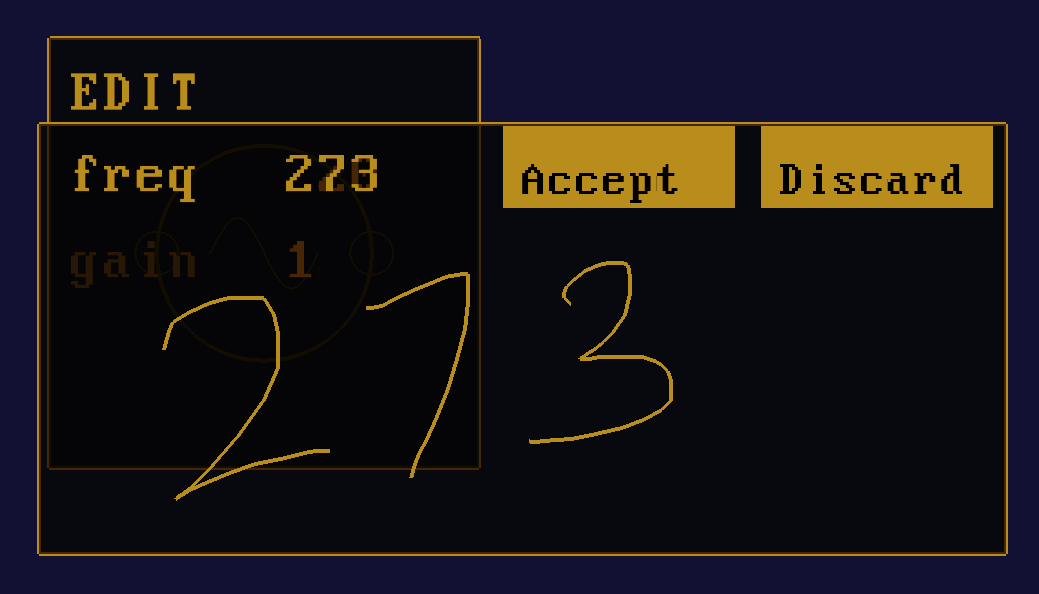
\includegraphics[width=0.45\textwidth]{figures/editor.png}
	\caption{Modifying the ``freq'' parameter of a unit generator with handwritten numeric input.}
	\label{fig:editor}
\end{figure}

Every base object may have inputs, an output, or both. These appear visually as small circles, or \emph{nodes}, on the perimeter of the object. 
Drawing a stroke from an input node to an output node, or vice-versa, forms a connection between those two objects. 
For example, connecting a sawtooth object's output to the \texttt{freq} input of a sine object creates a simple FM (frequency modulation) patch, with the sine as the carrier wave and the sawtooth as the modulator. 
Most objects only have one output source, but an input node may have several destinations within that object (e.g. frequency, amplitude, or phase of a given oscillator). 
In such cases, a pop-up menu appears from the node to display the options a user may have for the input destination. 

Objects and freehand drawings can be moved around on the canvas by touching and dragging them, a familiar gesture in the touchscreen software ecosystem. 
While dragging an object, moving the pen over a delete icon in the corner of the screen will remove that object, along with destroying any connections between it and other objects. 
Connections can be removed by grabbing them with a touch and then dragging them until they ``break.''
The entire canvas may be scrolled through using a two-finger touch, allowing for patches that extend well beyond the space of the tablet's screen. 

\begin{figure}[h]
	\centering
		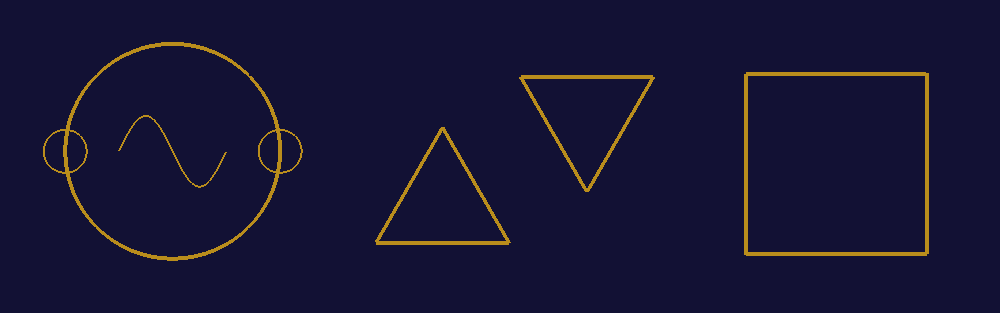
\includegraphics[width=0.45\textwidth]{figures/baseobjects.png}
	\caption{Base objects (left to right): unit generator, output, input, control-rate processor.}
	\label{fig:baseObjects}
\end{figure}

Four base types of objects can be drawn to the main canvas: audio-rate processors (unit generators; represented by a circle), control-rate processors (represented by a square), inputs (a downward-pointing triangle), and outputs (an upward triangle) (Figure \ref{fig:baseObjects}). 
Unit generators currently available include basic oscillators (sine, sawtooth, square, and triangle waves) and filters (resonant low-pass, high-pass, band-pass). 
Control-rate processors include a timer. 
Inputs and outputs are not currently implemented. 
After creating a base object, a menu opens to allow the user to select an object sub-type (see Figure \ref{fig:objectMenu}). Selecting a subtype from this menu creates an instance of that object, which may be then parameterized and connected to other objects. 

\begin{figure}[h]
	\centering
		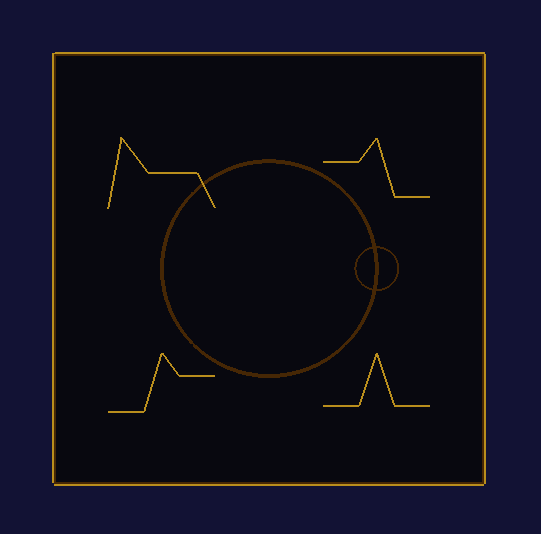
\includegraphics[width=0.35\textwidth]{figures/menu.png}
	\caption{Menu for selecting an object sub-type. Here, we see a menu for a unit generator object, showing ADSR, low-pass filter, high-pass filter, and band-pass-filter sub-types. Scrolling the menu will reveal additional sub-types.}
	\label{fig:objectMenu}
\end{figure}

\subsection{Handwriting Recognition}
\label{sec:HandwritingRecognition}

The concepts presented herein are generally invariant to the underlying algorithms and framework for handwriting recognition, but these topics merit discussion with regards to our own implementation in Auraglyph. 
The handwriting recognition engine used by Auraglyph is LipiTk~\cite{madhvanath2007lipitk}, a comprehensive open-source project for handwriting recognition research. 
LipiTk is not natively designed to function with iPad applications, but we extended it to do so with straightforward code changes and additions. 

LipiTk's default configuration uses dynamic time warping (DTW)~\cite{niels2005using} and nearest-neighbor classification (k-NN) to match pen strokes to a pre-existing training set of possible figures. 
The result of this procedure is one or more ``most likely'' matches along with confidence ratings for each match. 
We have found the speed and accuracy of LipiTk in this configuration to be satisfactory for real-time usage, though a slight, noticeable delay exists between finishing a stroke and the successful recognition of that stroke. 

Before they can be used to classify figures of unknown types, the recognition algorithms incorporated into LipiTk must be primed with a set of ``training examples'' for each possible figure to be matched. 
This training set is typically created by test users before the software is released, who draw multiple renditions of each figure into a specialized training program. 
This training program serializes the salient features of each figure into a database, which is distributed with the application itself. 

In our experience, LipiTk's recognition accuracy is highly linked to the quality, size, and diversity of the training set. 
For instance, a version of our handwriting database trained solely by right-handed users suffered reduced accuracy when used by a left-handed user. 
A comprehensive training set would need to encompass strokes from a range of individuals of varying handedness and writing style. 
Interestingly, though, LipiTk's algorithms are able to adapt dynamically to new training examples. 
An advanced system might gradually adjust to a particular user's handwriting eccentricities over time, forming an organically personalized software interaction. 
Auraglyph takes advantage of this feature to a small degree, allowing a user to add new training strokes via a separate training interface. 

However, as Auraglyph's interactions grow in sophistication and depth, the requirements of the handwriting recognition system may extend beyond what LipiTk innately provides. 
It is foreseeable that LipiTk's functionality may need to be wrapped into a higher level handwriting parser, aggregating individual characters into larger structures. 
For example, additional logic would need to classify the geometric arrangement of written text characters if they are to be used to represent programming constructs. 
Similarly, it is not clear if LipiTk's classifiers would be able to recognize ``filled-in'' areas in figures, such as the head of a quarter note. 
Additional research may be necessary to determine an effective solution to these and other issues. 

\section{Conclusions}
\label{sec:Conclusions}

I believe that using stylus control and multitouch manual input on touchscreen devices presents a number of novel opportunities for developing music computing interfaces. 
I have proposed a number of interactions to explore as part of an initial mapping of this space, within the context of an iPad application, code-named Auraglyph. 
I have further proposed methods for evaluating the success of individual interactions and the system as a whole. 
While building this system will require overcoming a number of design and technical obstacles, I am confident my experience at CCRMA and elsewhere has more than sufficiently prepared me for undertaking these tasks. 

%\end{document}  % This is where a 'short' article might terminate

%
% The following two commands are all you need in the
% initial runs of your .tex file to
% produce the bibliography for the citations in your paper.
\bibliographystyle{abbrv}
\bibliography{omni}  % sigproc.bib is the name of the Bibliography in this case
% You must have a proper ".bib" file
%  and remember to run:
% latex bibtex latex latex
% to resolve all references
%
% ACM needs 'a single self-contained file'!
%

%\balancecolumns 

% That's all folks!
\end{document}
